\chapter[SM SysId of LTI systems with EIV noise structure]{Set-Membership SysId of LTI systems with Errors-In-Variables (EIV) noise structure}

We have seen in the last chapter that an equation-error noise structure leads to a solution of LP problems for obtaining the Parameter Uncertainty Intervals, however, we have seen that there are some drawbacks. 
First of all the way we can find a bound $\Delta_e$ on the noise samples.
Then, the objective here is to find a way for dealing with the 'original' problem, that is the one using the output and input samples corrupted by noise. In order to gradually present all the needed ingredients for properly solving the problem, we show in turn general teoretical results and examples in which such results are applied to our problem of \textit{System Identification}.

\section{ Feasible Parameter Set in the EIV set-up}
In order to define also for this type of set-up the feasible parameter set, we have to follow the same road as we have done before. In particular we have to put together:
\begin{description}
    \itemsep-0.2em
    \item[A-priori information on the system] We know that the system belongs to a certain class $\mathcal{F}$, moreover we know the order $n$ of the system itself.
    \item[A-priori information on the noise] In particular the way the uncertainty enters the identification problem (we assume here the most general case when both input and output are corrupted by noise) and the boundedness of the noise samples, in particular
    \begin{equation}
        \vert \eta(k) \vert \le \Delta_\eta \quad
        \vert \xi(k) \vert \le \Delta_\xi
        \quad
        \forall k=1,...,N
    \end{equation}
    \item[A-posteriori information] They are nothing but the experimentally collected data $$\tilde{y}(k)=y(k)+\eta(k), \quad 
    \tilde{u}(k)=u(k)+\xi(k) $$
\end{description}
For an \textbf{LTI system of order $n$} the feasible parameter set is defined as follows: 

\begin{equation}\label{eq:FPS}
    \begin{aligned}
        \mathcal{D}_\theta = \{
            &\theta\in\mathbb{R}^p:  
            (\tilde{y}(k)-\eta(k))+\sum_{i=1}^n{\theta_i}\ ({y}(k-i)-\eta(k-i))=\\
            &\sum_{j=0}^m \theta_j \ (u(k-j)-\xi(k-j)), \quad
            k=n+1,...,N
        \} 
    \end{aligned}
\end{equation}
\noindent
In this context the definition of PUI is always the same, and the extrema of such an interval are defined as before by  solving the optimization problems:

\begin{equation*}
    \underline{\theta}_j = \min_{\theta\in\mathcal{D}_\theta} \theta_j, \quad 
    \overline{\theta}_j = \max_{\theta\in\mathcal{D}_\theta} \theta_j
    \Longrightarrow PUI_{\theta_j}=[\underline{\theta}_j,\overline{\theta}_j]
\end{equation*}
At this point the question is: \textbf{what type of $\mathcal{D}_\theta$ I obtain?} 
\section{Extended Feasible Parameter Set $\mathcal{D}_{\theta,\eta,\xi}$}
How we are able to see in the (\ref{eq:FPS}) the set definition depends also on the noise samples. The difference here is that I cannot eliminate them without adding any approximation. Substancially, I am introducing a non trivial number of new unknown in the description of the set: for $N$ collected samples, $2N$ new variables are added, which cannot be eliminated. For this reason we have to \textit{enlarge} the set $\mathcal{D}_\theta$ involving also the new variables. In this way we introduce the so-called \textbf{Extended Feasible Parameter Set (EFPS)} which we indicate with $\mathcal{D}_{\theta,\eta,\xi}$. \\
In order to better understand this aspect, let us consider a toy-example in which we have a single parameter $\eta(1)$ which is added to the pair $\theta_1, \theta_2$. The EFPS in this case -- how the figure below shows -- is a subset of $\mathbb{R}^3$.
\vspace{-0.2cm}
\begin{figure}[h]
    \centering
    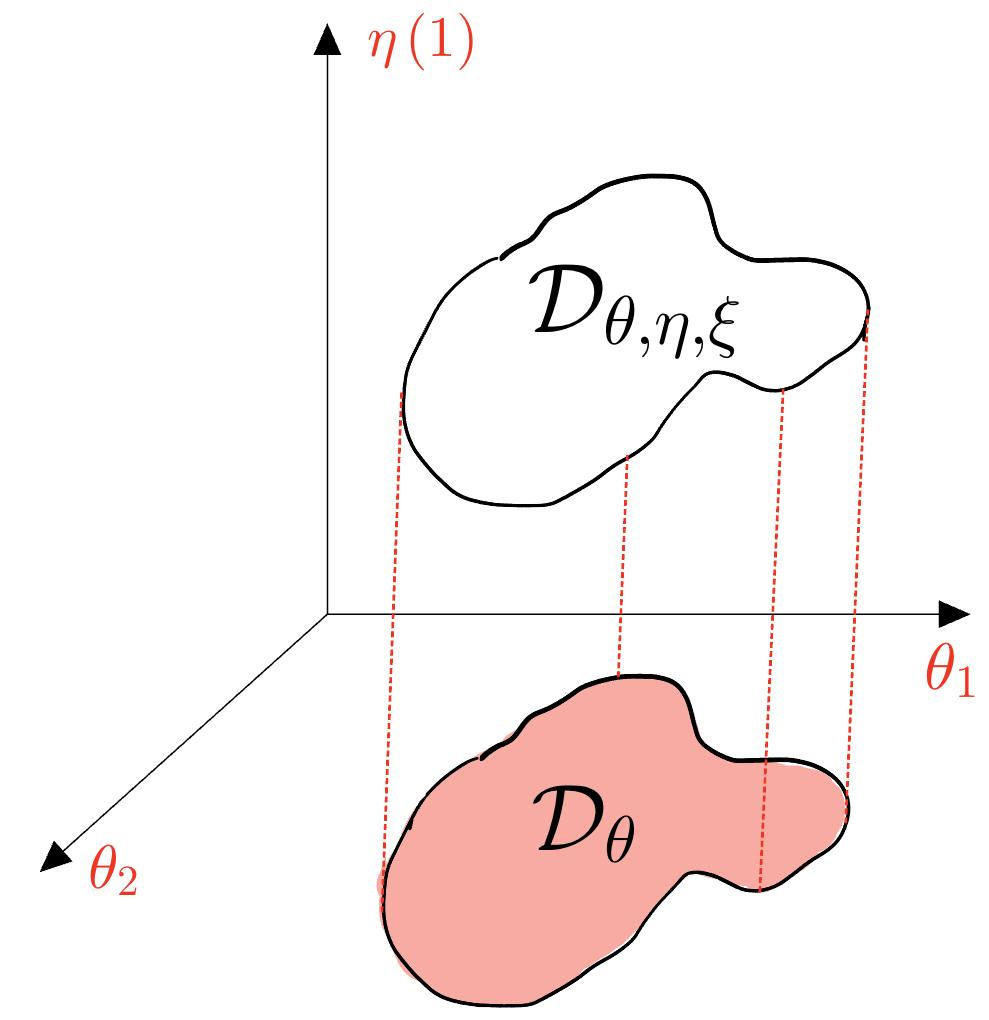
\includegraphics[scale=0.15]{img/EFPS.jpeg}
    \caption{Example in $\mathbb{R}^3$ of the Extended feasible parameter set}
\end{figure}

\noindent
The FPS $\mathcal{D}_\theta$ is nothing but the projection on the $(\theta_1,\theta_2)$ plane of the set $\mathcal{D}_{\theta,\eta}$, in this case no parameter $\xi$ is present.

\noindent
The definition of the \textbf{Extended Feasible Parameter Set} becomes the following:
\begin{equation}
    \begin{aligned}
        \mathcal{D}_{\theta,\eta,\xi} = \{
            &\theta\in\mathbb{R}^p, \eta\in\mathbb{R}^N, \xi \in \mathbb{R}^N: 
            \tilde{y}(k)-\eta(k) + \theta_1 (y(k-1)-\eta(k-1)) +\\
            &+\theta_2 (y(k-2)-\eta(k-2))+\dots+\theta_n (y(k-n)-\eta(k-n))=\\
            &=\theta_{n+1} (u(k)-\xi(k))+\theta_{n+2} (u(k-1)-\xi(k-1)) + ...+\\
            &\theta_{n+m+1} (u(k-m)-\xi(k-m)), \quad k=n+1,...,N\\
             &\vert \xi(k) \vert \le \Delta_\xi, \quad 
            \vert \eta(k) \vert \le \Delta_\eta, \quad k=1,...,N
        \}
    \end{aligned}
\end{equation}

\noindent
Such a set is defined by \textbf{nonlinear} and \textbf{non-convex} constraints and then the set is non-convex. In the specific case, the constraints that arises are \textbf{bilinear ones} which are a particular class of \textbf{polynomial constraints}. In general we know that is very hard to obtain a global minimum from a non-convex optimization problem, in this case using some tools for \textit{polynomial optimization} it is possible to reach a global minimum.\\

\noindent
In this framework the problem of finding the PUIs becomes:
{\large{
    \begin{equation}
        PUI_{\theta_j} = [\underline{\theta}_j,\overline{\theta}_j] \Longrightarrow 
        \underline{\theta}_j = \min_{\theta\in\mathcal{D}_{\theta,\eta,\xi} } \theta_j,    \quad
        \overline{\theta}_j = \max_{\theta\in\mathcal{D}_{\theta,\eta,\xi}} \theta_j
    \end{equation}
}}

\section{Convex relaxation for Polynomial Optimization Problems (POPs)}
\begin{center}
    \textsf{
    In this section we will introduce some general theoretical results on polynomial optimization problems, that -- how we have seen -- are the ones arising in the definition of the extended feasible parameter set (EFPS). We will start by formulating them, we will analyze the type of sets they produce and finally we will introduce the concept of \textbf{convex relaxation}.}
\end{center}

\noindent 
Let us consider the following general optimization problem:
\begin{equation}
    \begin{aligned}
        \min_{x} &f_0(x)\\ 
        &\text{s.t.} \ f_k(x)\le{0} \quad k=1, ..., l\\
        &f_k(x)=0 \quad k=l+1,...,m
    \end{aligned}
\end{equation}
where $f_0$ and $f_k, \ k=1,...,m$ are \textbf{multivariate polynomials} in the optimization variable $x$. Giving an example if $x=[x_1\ x_2\ x_3]^T$, an example of $f_0$ is
\begin{equation*}
    f_0(x)=x_1^2+x_2{x_3^3}+x_1^5{x_2^3}+7{x_3^2}
\end{equation*}
All POPs can be written, for sure, in the so-called \textbf{epigraphic form} by introducing a scalar (slack) variable $\gamma$.

\begin{multicols}{2}
    \noindent
    \textbf{\color{red}Original formulation}
    \begin{equation}
        \begin{aligned}
            \min_{x\in\mathbb{R}^n} &\ f_0(x)\\ 
            &\text{s.t.} \ f_k(x)\le{0} \quad k=1, ..., l\\
            &f_k(x)=0 \quad k=l+1,...,m
        \end{aligned}
    \end{equation}
    \newcolumn\\
    \textbf{\color{red}Epigraphic formulation}
    \begin{equation}
        \begin{aligned}
            \min_{x\in\mathbb{R}^n, \gamma \in \mathbb{R}} &\ \gamma\\ 
            &\text{s.t.} \ f_0(x)\le\gamma\\
            &f_k(x)\le{0} \quad k=1, ..., l\\
            &f_k(x)=0 \quad k=l+1,...,m
        \end{aligned}
    \end{equation}
\end{multicols}
\noindent
By rewriting a generic POP in the epigraphic form, it becomes a problem of \textbf{minimizing a linear function over a non-convex set described by polynomial constraints} (this is also true  for the unconstrained case).

\begin{figure}[h] \label{fig:non-convex}
    \centering
    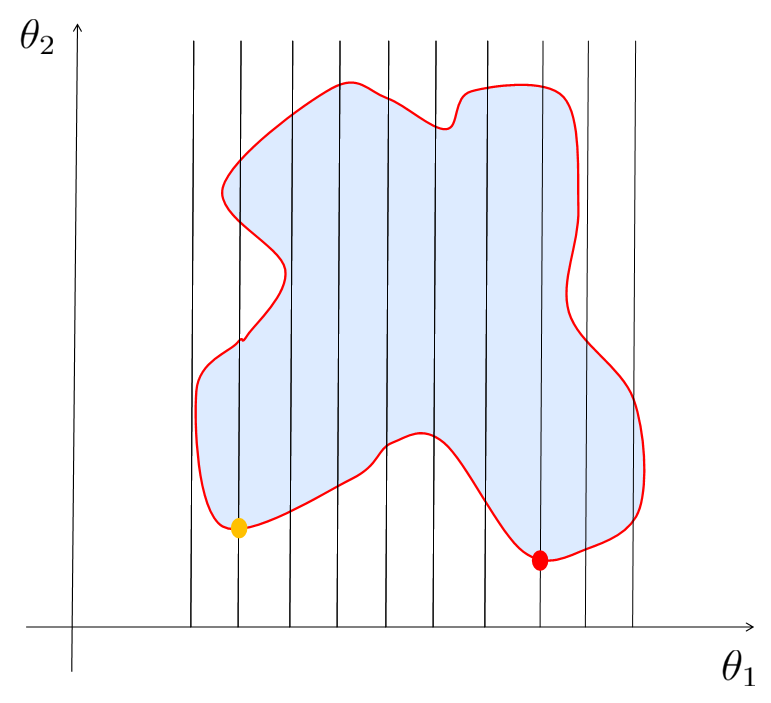
\includegraphics[scale=0.5]{img/nonconvex.png}
    \caption{Example of min a linear objective (thin line) over a non-convex set (sky-blue)}
\end{figure}

The figure (\ref{fig:non-convex}) shows the general idea. We are moving a linear objective (thin lines in black) over the set in sky-blue derived by the polynomial (so non-convex) constraints. The thin lines are the so-called \textit{level-curves} in order to minimize $\theta_1$. Moreover the orange point is a \textbf{local minimum}, while the red one is the \textbf{global minimum}.\\

\noindent
\textbf{\color{red}Important remark:} since a generic POP can written in epigrapigh form, we can note that the non-convexity of  the problem is now \textbf{completely embedded} in the description of the set of constraints $\to$ whether we want to compute the \textbf{global optimal solution} we have to deal with the non-convexity of the set of constraints. It is very high the probability of getting stuck in local minima.\\

\begin{definition}[Convex hull of a non-convex set] Given a non-convex set $\mathcal{S}$, the \textbf{convex hull} for it is the smallest  convex-set including $\mathcal{S}$. 
\end{definition}

A very-nice property is that the \textbf{min/max} computed on the convex hull is equal to the one computed on the original set. In this way we gain the convexity of the problem. 

In other words,if we are able to write down the equations describing the convex hull $C_\mathcal{S}$ of the non-convex set $\mathcal{S}$ we have that:
\begin{equation}
    \min_{x\in{C_\mathcal{S}}} f(x) = \min_{x\in\mathcal{S}} f(x)
\end{equation}
The drawback here is that, in general, obtaining a mathematical description of $C_\mathcal{S}$ is a quite difficult problem.\\
In the particular case of POPs, it is possible to compute a \textbf{convex relaxation os $\mathcal{S}$} depending on a parameter called the \textbf{order of relaxation} $\delta$.

\begin{figure}[h]
    \centering
    \subfigure[Convex hull $C_\mathcal{S}$]{
        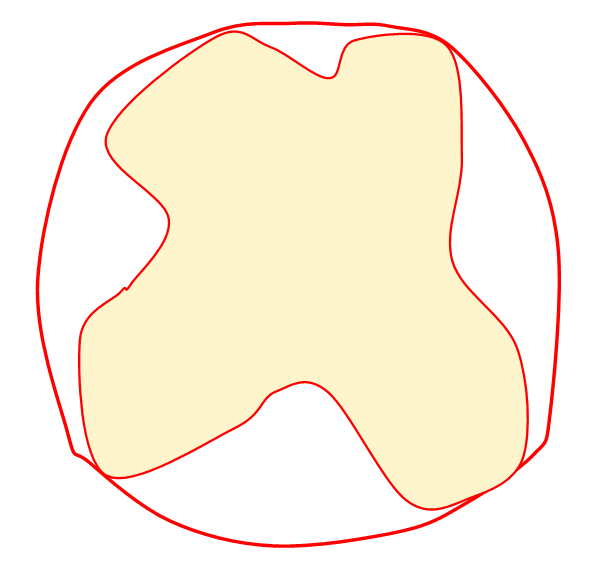
\includegraphics[scale=0.5]{img/convex_hul..png}
    }
    \subfigure[Relaxing the convex hull by $\delta$]{
        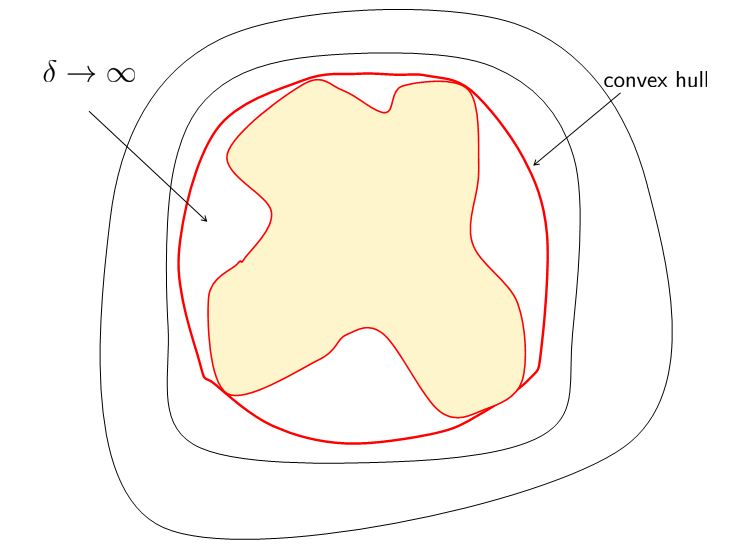
\includegraphics[scale=0.5]{img/relax.png}
    }
\end{figure}
\begin{figure}[h]
    \centering    
\end{figure}

For a given $\delta$ we have different relaxed sets as you can see in the figure, moreover for $\delta\to\infty$ the relaxed set coincides with the convex hull in red.\\
All of this concepts are then applied to our optimization problem which is aimed to find the extrema of the Parameter Uncertainty Intervals for our problem of System Identification. In this case comes up an interesting property, that is, for sure whatever is the order $\delta$, we are including the real PUI. More specifically, we have that for each $k$ the relaxed solutions $\underline{\theta}_k^{\delta}$ and $\overline{\theta}_k^{\delta}$ are such that:
{\large{
    \begin{equation}
        \underline{\theta}_k^{\delta} \le \underline{\theta}_k
        \quad 
        \overline{\theta}_k^{\delta} \le \overline{\theta}_k
    \end{equation}
}}
moreover it holds that: 
\begin{equation}
    \lim_{\delta\to\infty} \underline{\theta}_k^{\delta} = \underline{\theta}_k \quad
    \lim_{\delta\to\infty} \overline{\theta}_k^{\delta} = \overline{\theta}_k
\end{equation}

In order to solve a POP by means of \textit{Lassere convex  relaxation approach} in MATLAB we use:
\begin{enumerate}
    \item \textsf{SparsePOP} that given a polynomial optimization problem and the order of relaxation $\delta$ provides a \textit{Semidefinite relaxed problem (SDP)};
    \item Finally \textsf{SparsePOP} calls the optimization toolbox \textsf{SeDuMi} which solves  the given SDP. 
\end{enumerate}
 


